\documentclass[a4paper]{article}

\usepackage{soulutf8}
\usepackage{graphicx}

\usepackage[utf8]{inputenc} % Кодировка UTF-8
\usepackage[russian]{babel} % Поддержка русского языка
\usepackage{amsmath,amssymb}

\usepackage{blindtext}
\usepackage{multicol}

\usepackage{geometry}
\geometry{left=15mm}
\geometry{right=15mm}
\geometry{top=25mm}
\geometry{bottom=25mm}

\usepackage{makecell}
\usepackage{lettrine}
\usepackage{eso-pic}

\usepackage[absolute,overlay]{textpos}
\usepackage{rotating}

\usepackage{fancyhdr} 

\renewcommand{\LARGE}{\fontsize{25}{40pt}\selectfont}
\renewcommand{\large}{\fontsize{16}{16pt}\selectfont}

\parindent=5cm
\usepackage{multirow}% http://ctan.org/pkg/multirow


\begin{document}
\linespread{1.6}

\fontsize{15}{15pt}\selectfont 
\begin{center}
Федеральное государственное автономное образовательное учреждение высшего \\образования «Национальный исследовательский университет ИТМО»\\
Факультет программной инженерии и компьютерной техники\\
\vspace{7cm}
Лабораторная работа №6\\
\large{\textbf{Работа с системой
компьютерной вёрстки \TeX
}}\\
\fontsize{13}{13pt}\selectfont 
Вариант №15\\

\vspace{7cm}
\end{center}
\begin{flushright}
Выполнил \\
Макогон Ярослав Вадимович \\
Номер группы: P3118\\
Проверилa\\
Малышева Т. А.\\

\end{flushright}


\newpage
\linespread{1}
\fontsize{9}{10pt}\selectfont 

\setcounter{page}{8}
\pagestyle{fancy} 
\fancyhf{}
\fancyhead[L]{
\begin{flushleft}
    \textbf{\thepage} \hspace{0.5cm} \begin{minipage}[b]{0.90\textwidth}\centering \so{КВАНТ.1997/№6}\end{minipage}
\end{flushleft}
}
\renewcommand{\headrulewidth}{0pt}



\begin{multicols}{3}
    \begin{flushright}
        \textit{Таблица}
    \vspace{-2.4mm}
    \end{flushright}
    \begin{tabular}{|p{2mm}|p{7.6mm}|p{7.6mm}|p{11mm}|p{8.6mm}|} \hline
    \multicolumn{5}{|c|}{\textbf{Удар «средней силы»}}\\[5pt]  \hline
     & $m$(кг) & $h$(м) & $E_k$(Дж) & $F$(кН) \\ \hline
     \multirow{2}{*}{R}
    & 0,5 & 1,0 & 5 & 25 \\
    & 1,0 & 1,0 & 10 & 100 \\ \hline
    \end{tabular} 
    \hspace{-17pt}
    \begin{tabular}{|p{2mm}|p{10mm}|p{13mm}|p{16mm}|}
    \multicolumn{4}{|c|}{\textbf{Удар «со всего плеча»}} \\ [5pt] \hline
     & $L$(м) & $E_k$(Дж) & $F$(кН) \\ \hline
    M. & 40 & 100 & 100 \\
    K. & 20 & 1000 & 300 \\ \hline
    \end{tabular}\vspace{15pt}
горизонту, равна
$$L = \frac{u_0^2}{g} sin 2\alpha = \frac{u_0^2}{g},$$
поэтому

$$E_k = \frac{mu_0^2}{2} = \frac{mgL}{2}.$$

В таблицу мы записали оценки ки- нетической энергии обычного молот- ка (М.) и кувалды (К.) для ударов «средней силы» и «со всего плеча». Туда же мы занесли и вычисленные значения максимальной силы ($F$). Из таблицы видно, что даже при ударе «средней силы» силы вполне хватает. Аналогично обстоит дело и с другими гвоздями. «Запас силы» довольно значителен, особенно для гвоздей малых размеров, и в случае удара кувалдой «со всего плеча» на два порядка превышает максималь- ное значение силы сопротивления. \\
Справедливости ради отметим, что в действительности такие силы возникнут лишь в том случае, если гвоздь упирается в материал гораздо более жесткий, чем сталь. При забивании гвоздя в дерево фактически работают
две последовательно включенные пружины: гвоздь и дерево$^1$. Так что общая жесткость этой системы пружин равна

$$k = \frac{k_1k_2}{k_1 + k_2}.$$
Однако, и в этом случае запас силы существенный. Действительно, для \\

\noindent\rule{0.5\linewidth}{1pt} \\
\vskip -5pt

$^1"$\textit{Справедливости ради» отметим, что молоток -- тоже колебательная система, и время прохождения волны вдоль молотка и обратно сильно влияет на качество удара. Так что у нас не две пружины, а три. Кроме того, конец гвоздя при каждом ударе углубляется в дерево, и сила сопротивления при этом меняется слабо. Поэтому дерево не совсем пружина. Но при численных оценках \textit{с запасом} эти факторы не очень существенны. \textbf{(Прим. ред.)}} \\
учета смягчающего действия дерева оценим его жесткость формулой
$$k = E_\text{д}.R$$
Возможность такой оценки видна из следующих рассуждений. Вообще говоря, «деревянная пружина» у нас очень странная полупространство, заполненное деревом. Но при надав- ливании гвоздя существенным обра- зом деформируется не все полупро- странство, а лишь полусферическая область вблизи острия гвоздя, кото- рая больше похожа на стандартную пружину. Пространственный масш- таб у нас один
радиус гвоздя $R$,
поэтому естественно оценить длину этой области как $R$, а площадь как
$R^2$. Отсюда и получается выписан- ная нами формула. Приняв модуль Юнга для дерева $E_\text{д} = 5 \cdot10^{10} Па$, для
удара молотком «со всего плеча» по комбинированной пружине получим
\begin{equation}
    \label{fval}
    F = 80 \text{ кН},
\end{equation}
чего по-прежнему вполне достаточно (\ref{fval}).

Итак, с силой проблем нет.

Рассмотрим второй аргумент «против» - «энергии не хватит». В этом случае убедиться в обратном достаточно просто. Для того чтобы забить гвоздь, энергия молотка должна превышать значение
$$E_{min} = A_{\text{тр}}+E_{p1} + E_{p2},$$
где $A_{\text{тр}} = (F_0+ F_{max})l_0/2$
-
работа
против силы трения, $Е_{p12}$ - потенциальные энергии деформированных дерева и гвоздя. Первое слагаемое гораздо больше двух остальных. Например, для потенциальной энергии сжатия гвоздя можно записать

\begin{multline*}
E_{p2} = \frac{\sigma^2}{2E}V \approx \frac{F_{\text{max}}}{SE} \frac{F_{\text{max}}}{2S} l_0 S \\
\approx \frac{F_{\text{max}}}{SE} A_{\text{тр}} \ll A_{\text{тр}}.
\end{multline*}
Поэтому для забивания гвоздя доста- точно, чтобы энергии молотка хватило, для преодоления силы трения. Для эталонного гвоздя это составляет в случае ели 70 Дж, в случае бука -- 400 Дж.

Таким образом, удара кувалдой должно хватить.

Так же оптимистично выглядят результаты расчета и для стандартных гвоздей (рис.5). В случае ели проблемы могут возникнуть лишь с вбиванием «двухсотки». Для бука энергии требуется побольше, но даже для



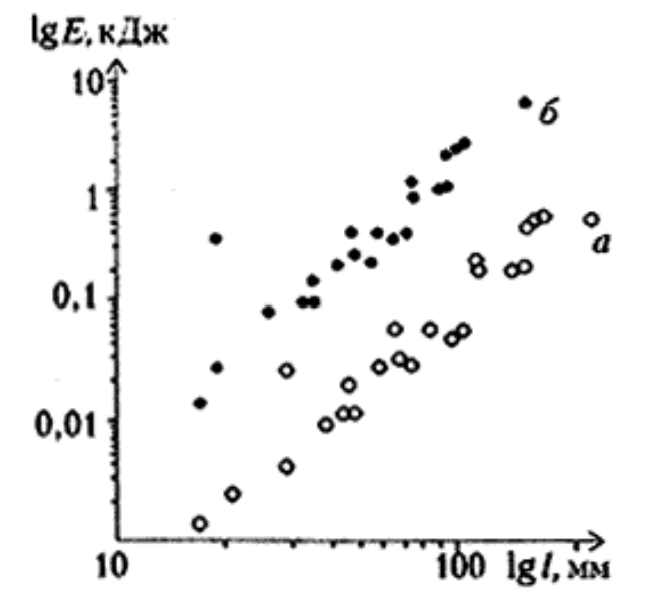
\includegraphics[width=1\linewidth]{imageg} 
{\textbf{\textit{Рис. 5. Энергии, необходимые для вдавливания гвоздей (а - ель, б - бук)}}}
\vspace{10pt}\\
«соток» соответствующие значения порядка 1000 Дж.
\vspace{2pt}
\noindent\rule{1\linewidth}{1pt} \\
\textsf{{\Large{Последний и окончательный аргумент}}} 
\vskip -7pt
\noindent\rule{1\linewidth}{1pt} \\
Не обнаружив явных причин, запрещающих вбивать гвозди с одного удара, мы вернулись к эксперименту. Стали забивать гвозди, не жалея сил. И очень скоро все прояснилось. То, что раньше мы списывали на неудачу при сильном ударе гвозди не забивались в бук, а просто гнулись, - и есть главное. Научное название этого эффекта неустойчивость Эйлера. 

Обычно неустойчивость Эйлера демонстрируют следующим образом. Пусть на шарнирно закрепленный стержень действует сила $F$ (рис.6). Пока эта сила невелика, гвоздь прекрасно выдерживает нагрузку. Но как только сила превысит критическое значение
$$F_{\text{кр}} = \frac{\pi^2EI}{l^2},$$
стержень становится неустойчивым. Малейший его изгиб начинает катастрофически расти с ростом силы, и стержень ломается. (Такое поведе ние стержня само по себе удивитель но. Оно совсем не похоже на обычное поведение упругих тел, к которому Мы привыкли, деформации постепенно увеличиваются с ростом при- ложенной силы. Обсуждение причины этого увело бы нас в сторону, поэтому ограничимся лишь замечанием, что связано это с экстремальным свойством отрезка прямой - он короче любой другой линии, соеди няющей две точки.)

Величины, входящие в выражение для критической силы, могут быть

\end{multicols}


\end{document}

% Увеличить параграф \parindent=2cm
% Подписать формулы и сослаться в тексте equation
% Объеденить столбцы в таблице \multirow{2}{*}{R}